\section{Vista de desarrollo}

Para la realización del trabajo se propone utilizar como herramienta de desarrollo el IDE de programación Visual Studio 2010 Express o cualquiera de sus versiones posteriores, pues se trabajará con el SDK oficial de Microsoft Kinect.
En esta vista encontramos los diagramas de componentes tanto de la aplicación Entrenador el cual se muestra en la Figura \ref{fig:Co_Entrenador} \nameref{fig:Co_Entrenador}, como de la aplicación Practicante el cual se muestra en la Figura \ref{fig:Co_Practicante} \nameref{fig:Co_Practicante}, mostrando de manera general cada una de las partes en que están compuestas dichas aplicaciones.

\subsection{Diagrama de componentes}

\begin{figure}[H]
	\begin{center}
		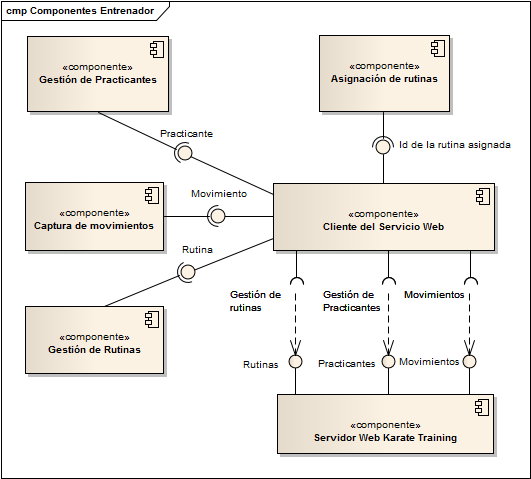
\includegraphics[scale=0.8]{./Figuras/Arquitectura/Componentes_Entrenador}
	\end{center}
	\caption{Diagrama de componentes - Entrenador}
	\label{fig:Co_Entrenador}
\end{figure}

\clearpage

\begin{figure}[H]
	\begin{center}
		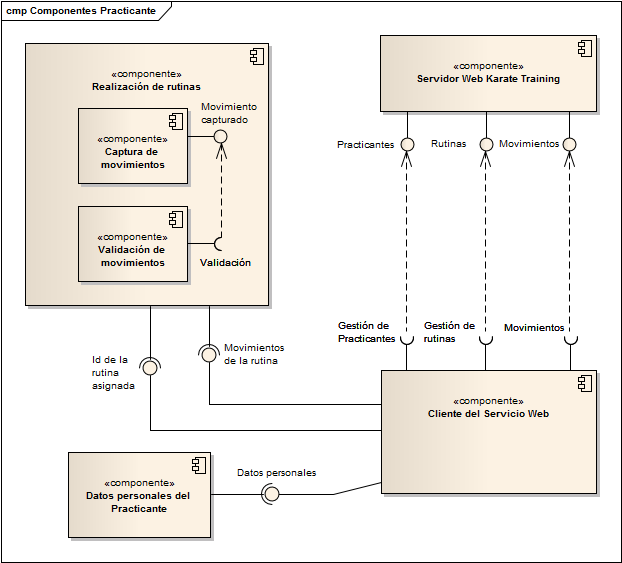
\includegraphics[scale=0.8]{./Figuras/Arquitectura/Componentes_Practicante}
	\end{center}
	\caption{Diagrama de componentes - Practicante}
	\label{fig:Co_Practicante}
\end{figure}

\clearpage